\chapter{TnT Server}
TnT Server is the core of OptoFidelity TOUCH robot systems. It provides functionalities for touch and test applications such as controlling robot and taking camera images. The component is called server because to achieve this functionality it acts as a HTTP server.

\section{Installing/re-installing the Server}
\label{sec:server_installation}

When installing an update to TnT Server, or re-installation is needed, OptoFidelity Technical Support can perform the operation assuming TeamViewer access to the PC is available. See the "Support" section \ref{part:support} for details how to request support.

If you have an installer package available, and want to perform the installation independently, please follow these instruction carefully.

Installation can be done by running the installation package. To run the server a dedicated HASP USB encryption dongle has to be connected to the measurement PC.

\subsection{Windows}

A valid license text file has to be available with the following path: "\tntLicensePath".

The installer is a self-contained exe file which launches a wizard that will help the user through the installation process.

In case the user wants to re-install the Server, the following procedure should be followed in order to keep the configuration unchanged:
%
\begin{enumerate}
	\item \label{itm:server_first} Go to the folder "\tntRootPath" and create a back-up of existing "\tntServerFolder" folder by renaming the folder as "TnT Server 2020-01-02" where the date is the backup date.
	\item Run installation package as usual (the installer will create a new "\tntServerFolder" folder).
	\item Copy "configuration" folder from backup to the new installation.
	\item Under "configuration" folder there should be "client\_config.yaml". If any new features were added to the API, they should be exposed in the client by adding them to correct include lists in this config file. This step can usually only be performed by OptoFidelity personnel.
	\item Generate TnT Client that matches the new server installation. Instructions for this can be found under "\tntServerFolder/client/README.md".
	\item Copy "data" folder from backup to the new installation.
	\item When TnT Server is updated, also TnT UI must be updated to latest version. See Section \ref{sec:ui_installation} for instructions.
\end{enumerate}

After SW has been updated, carefully step through the pre-run checklist in Section \ref{sec:pre_run_checklist}.

\subsection{Macos}

A valid license text file has to be available with the following path: "\tntLicensePathMacos".

The installer is a shell script with embedded data and can be ran from command-line. Once executed, the installer will prompt user to continue installing the package.

In case the user wants to re-install the Server, the following procedure should be followed in order to keep the configuration unchanged:
%
\begin{enumerate}
	\item Run the installation script from any location. The installer will create a backup of existing installation and copy new files under "\tntRootPathMacos\tntServerFolder". 
	\item The configuration and data directories are automatically copied from the latest backup to the new location by the installer.
	\item TnT Client is automatically generated and installed to the global python environment by the installer.
	\item Under "configuration" folder there should be "client\_config.yaml". If any new features were added to the API, they should be exposed in the client by adding them to correct include lists in this config file. This step can usually only be performed by OptoFidelity personnel.
	\item If any changes to "client\_config.yaml" were made, manually generate TnT Client that matches the new server installation. Instructions for this can be found under "\tntServerFolder/client/README.md".
	\item When TnT Server is updated, also TnT UI must be updated to latest version. See Section \ref{sec:ui_installation} for instructions.
\end{enumerate}

After SW has been updated, carefully step through the pre-run checklist in Section \ref{sec:pre_run_checklist}.

\subsection{Pre-run checklist}
\label{sec:pre_run_checklist}

Depending on the content of the update, it is possible, that there are changes affecting some of the previously configured properties, for example positioning of the DUTs, or the lengths of the tools. Therefore it is not recommended to perform any updates entirely remotely. Instead, after software has been updated, the operator should be physically close to the robot to be able to use the emergency stop in case something has changed unexpectedly. Perform the following actions monitoring the robot carefully:
%
\begin{enumerate}
    \item Make sure that the tip attach status of the robot matches the status in the Tips view in the UI i.e. if a tip is attached to robot finger, it should be shown as such in the UI.
    \item Check that all the tips (including multifinger) are properly attached to their racks (in the back of their slots).
	\item Set low robot speed such as 20 mm/s from TnT UI and for each existing DUT, tap the four corners using the "Test Tap" button under DUT view in the UI.
	\item Pick and drop each positioned tip using the controls under Tips view in the UI to make sure that the slot positions are valid.
	\item In case of TPPT delivery: Run worst case lines in Swipe test and run Tap test with sparse grid e.g. 50 mm spacing. Please check that the data is received from DUT and that the gestures function correctly.
	\item In case of HSUF delivery, run a script where icon and text is detected on a DUT and the detected position is tapped.
\end{enumerate}

\section{Starting and closing the server}
\label{sec:server_start}
The server is ran by double clicking the server icon on the desktop. It is also possible to run the "\tntServerExecutable" directly. It can be found from the folder "\tntRootPath\tntServerFolder". The server should open a new terminal window (unless started directly from terminal when the program is run in the existing window). The terminal window shows the server log messages. After the software has started the user can see the following log message in the terminal window "Server ready at port 8000". Additionally, there should be no errors in the log messages. Errors are shown in red and as such they are easily visible when scrolling the terminal window. After server has been started successfully, the configuration that was used will be saved as a backup if there are differences when compared to previous backup. If everything has worked successfully you should see something like in Figure \ref{sec:server_start}.

\begin{figure}[h]
	\centering
	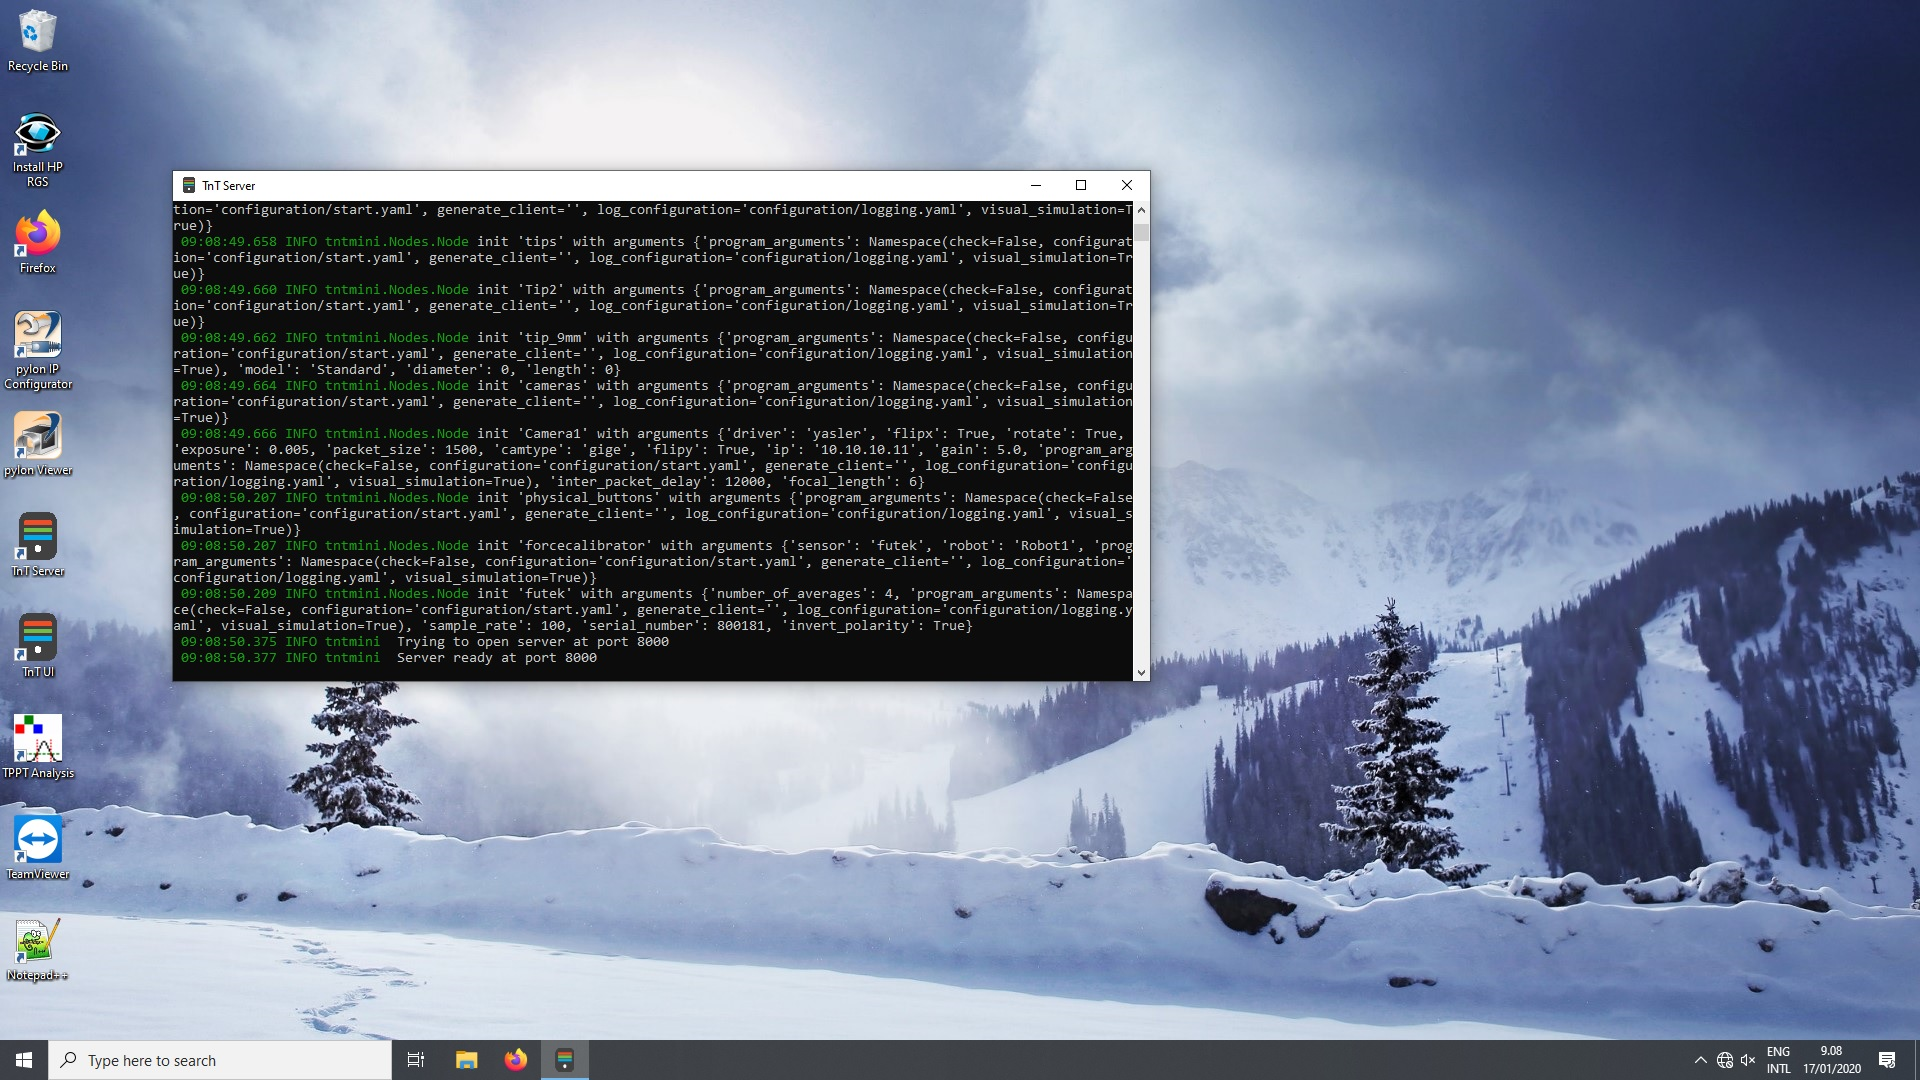
\includegraphics[width=0.7\linewidth]{server_start.jpg}
	\caption{PC after successful server initialization.}
	\label{fig:server_start}
\end{figure}

During a successful start sequence, the robot should home all the axes. This is done every time even though the robot might already be in the home position.

\subsection{Command-line arguments}

Following command-line arguments can be passed to \tntServerExecutable :

\begin{tabular}{ll}
 \texttt{--configuration=[path]} & Path to configuration file. \\
 & Default values is \texttt{"configuration/start.yaml"}. \\ 
\texttt{--configuration-ip=[ip]} & IP address of FTP server where configuration file can be obtained. \\ 
 & Default value is \texttt{"192.168.127.254".}\\
 \texttt{--fetch-configuration} & Fetch configuration file via FTP and save locally as file specified \\
  & by \texttt{--configuration}. Default value is \texttt{false}.\\
 \texttt{--push-configuration} & Push file specified by \texttt{--configuration} to FTP server. \\
  & Default value is \texttt{false}.\\
  \texttt{--log-configuration=[path]} & Path to logging configuration file. \\
  & Default value is \texttt{"configuration/logging.yaml"}.\\
  \texttt{--visual-simulation} & Use visual simulation if simulator is configured?\\
  & Default value is \texttt{true}.\\
  \texttt{--generate-client=[path]} & Generate TnT Client using provided path to client config file.\\
  & Not used by default.
\end{tabular} 

\section{Motion control and safety}

TnT Server is able to plan robot motion in 3D space for multi-axis robots. The robot axes are run synchronously to execute a planned trajectory. User can set the linear speed and acceleration of the robot effector that is used in the motion planning. Due to safety regulations, the software clamps the given speed to \textbf{250 mm/s}. Using speed higher than that requires special safety equipment which is not part of standard delivery. The acceleration specified by user is not limited by software but the individual robot axes have some limited acceleration which limit the effector acceleration.

\warningbox{Using high acceleration such as over 600 mm/s$^2$ requires a heavy-duty table for the robot to avoid wobbling followed by decreased system accuracy.}

The maximum speed and acceleration of individual axes of the robot are limited by several factors such as maximum current draw and voltage and varies between robots. After the trajectory has been planned with given effector speed and acceleration, the resulting axis speeds and accelerations are evaluated. If the maximum speed or acceleration of axes are violated, the duration of the trajectory is scaled so that then motion can be executed within axis capabilities. In this case a warning message is printed to TnT Server log and the motion is executed using smaller speed and acceleration that what user specified.

With synchro finger robot the rotation of azimuth axis while keeping effector stationary often involves x and y axis motion with very high acceleration even if the rotation is fairly slow. Hence, it is common that when azimuth rotation is involved, the software needs to slow down the motion from what user specified.

\warningbox{Even though the effector speed is clamped to 250 mm/s, the axes can move faster during motion if rotary axes are involved in synchronous motion with prismatic axes. Often the y-axis carries a lot of weight so user must be aware.}

\section{Simulator}

TnT Server can be run as simulator in the absence of physical robot. The simulator can be run in visual mode where the robot 3D model is used to visualize the motion or it can be run in non-visual mode where server just simulates the motion numerically and no visual feedback is given.

\warningbox{Simulator is currently intended mostly for development use so the usability is limited and setup is somewhat tricky.}

\subsection{Setting up simulator}

To run simulator with visualization, copy the directory containing required model STL files under

\texttt{\tntServerFolder/tntserver/web/model/}

For synchro robot, there should be a directory named \texttt{synchro\_asvcf}. The model files are not part of normal TnT Server build. They are provided separately if this has been approved as part of the delivery.

To start the server in simulation mode, the \texttt{start.yaml} configuration file under \texttt{\tntServerFolder/configuration/} must have following text at the beginning of the file:

\begin{lstlisting}
- name: tnt
  cls: TnT.TnT
  parent:
  connection:
  
- name: fileserver
  cls: NodeFileServer
  parent: tnt
  arguments:
    path: web
    port: 8010
  connection: tnt

- name: simulator
  cls: NodeSimulator
  parent: tnt
  connection: tnt
\end{lstlisting}

In normal configuration file there only exists the \texttt{tnt} part.

Additionally for node \texttt{Robot1} the value of argument \texttt{simulator} must be set \texttt{true} and value of \texttt{host} must be set to \texttt{127.0.0.1}. For node \texttt{Camera1} the value of argument \texttt{driver} must be set to \texttt{simulator}.

To illustrate only the relevant parts of the configuration file, it should look like following:

\begin{lstlisting}
- name: Robot1
  cls: Synchro.Robot
  parent: robots
  connection: Robot1_base
  arguments:
    host: 127.0.0.1
    port: 4001
    simulator: true
    
- name: Camera1
  cls: TnT.Camera
  parent: cameras
  connection: camera_mount
  arguments:
    driver: simulator
\end{lstlisting}

\subsection{Running numerical simulator}

To run simulator without visualization, TnT Server should be launched with following command:
\begin{lstlisting}
"TnT Server" --visual-simulation=false
\end{lstlisting}

This can be useful for testing that e.g. script execution works without errors without having to wait for the visualization to load.

\subsection{Running visual simulator}

When TnT Server is launched after the configuration changes without additional flags, the visualization should open in browser window and look something like in Figure \ref{fig:simulator}.

\begin{figure}[h]
	\centering
	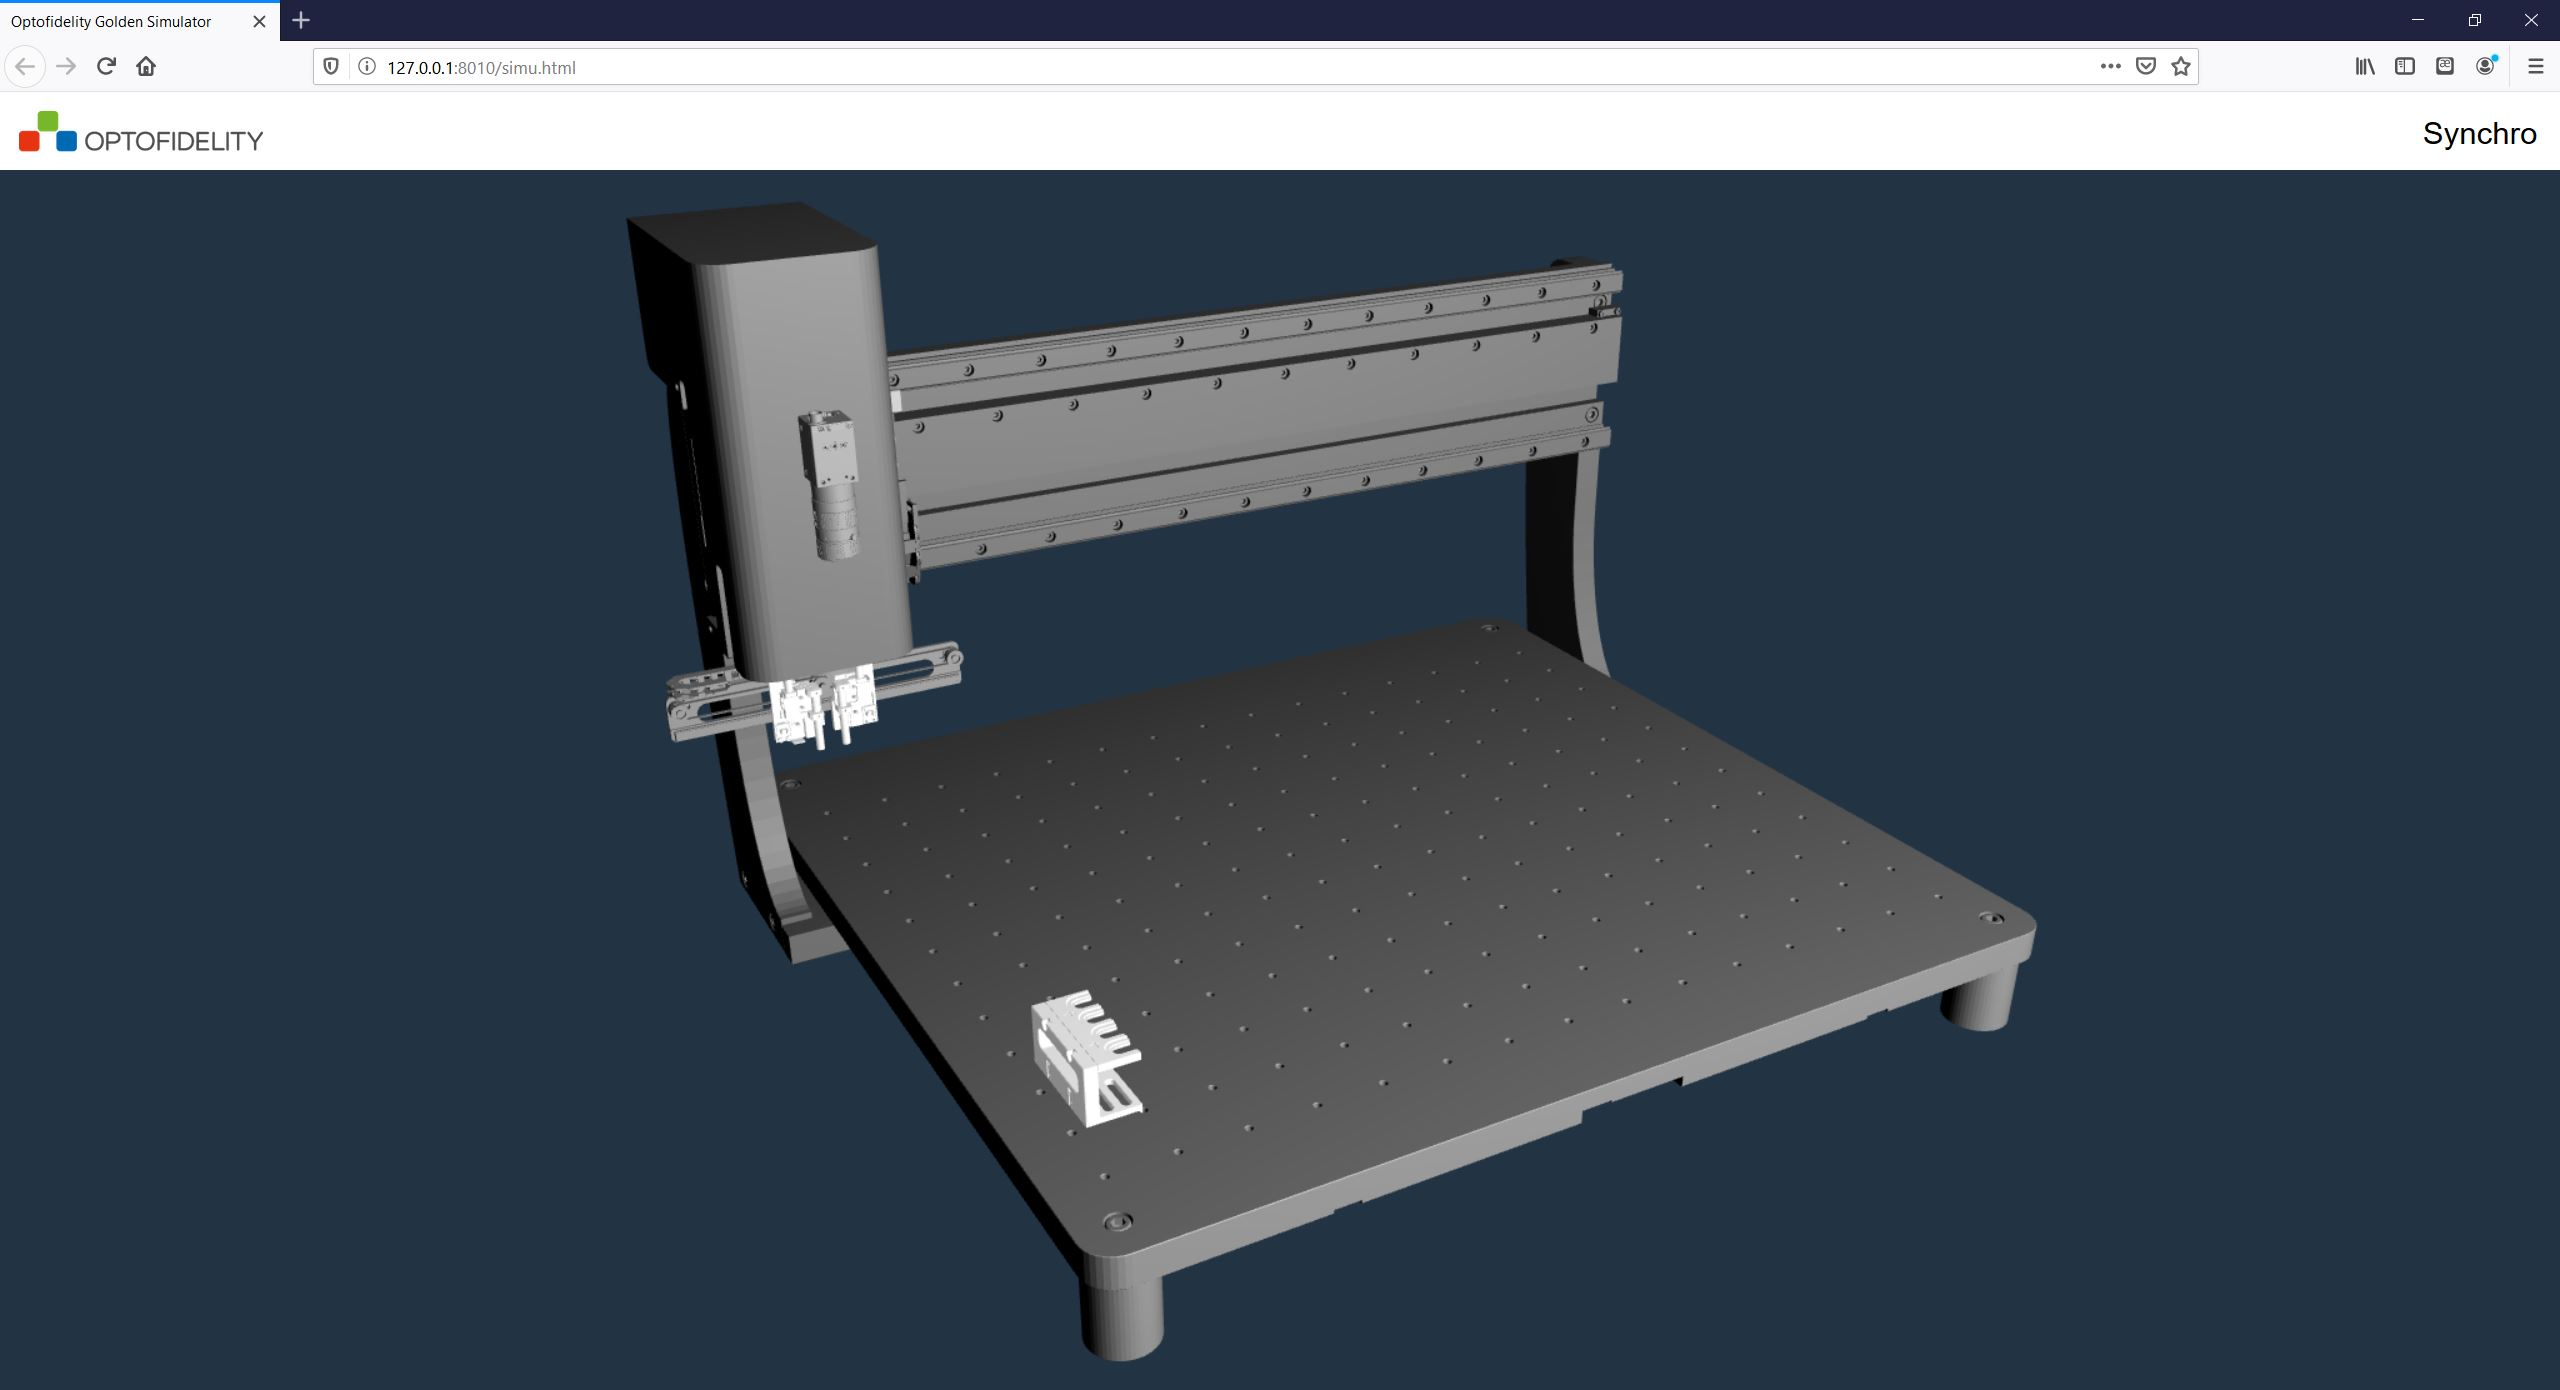
\includegraphics[width=0.7\linewidth]{simulator.jpg}
	\caption{Robot simulator visualization in browser window.}
	\label{fig:simulator}
\end{figure}

\notebox{Sometimes the browser will keep on loading the model for a long time. It may help if you stop the page loading and then refresh it.}

\notebox{The browser window must remain visible in the Windows workspace for the simulation to work. Otherwise motion commands will block forever.}

The view can be controlled by dragging cursor over it. Following controls apply:

\begin{itemize}
\item Left mouse button: rotate view
\item Right mouse button: pan view
\item Mouse wheel: zoom view
\end{itemize}


\subsection{Adding visual content to simulator}

To show a rectangular image object in simulator workspace, add following at the end of the configuration file

\begin{lstlisting}
- name: my_image_object
  cls: NodeSimulatorObject
  parent: ws
  arguments:
    enabled: true
    type: texture
    ppmm: 20
    position: [200, 250, 0, 0, 0, 0]
    image: my_image_file.png
    width: 50
    height: 100
    simulator_parent_object: table
  connection: ws
\end{lstlisting}

The arguments are as follows:

\begin{itemize}
\item \texttt{enabled}: Show object or not.
\item \texttt{type}: Type of simulator object. Value \texttt{texture} is image based texture.
\item \texttt{ppmm}: Pixels per millimeter. Affects the scaling of the object in the simulation workspace.
\item \texttt{position}: List of values \texttt{[pos\_x, pos\_y, pos\_z, euler\_x, euler\_y, euler\_z]}.
\item \texttt{image}: Path to image file relative to server installation directory.
\item \texttt{width}: Width of rectangle in workspace in mm.
\item \texttt{height}: Height of rectangle in workspace in mm.
\item \texttt{simulator\_parent\_object}: Name of parent to which is object is attached to.
\end{itemize}

You can define multiple objects as long as they have different names.

\section{Server troubleshooting}
In this section we have collected the most common issues encountered by our customers. In case you cannot find solution from here, please contact OptoFidelity support. More information about support can be found from Part \ref{part:support}.

\subsection{The terminal window opened during server start is suddenly closed by itself}

To see the error message that appears just before the terminal window shutdown, the user should run the "TnT Server.exe" directly as instructed in Section \ref{sec:server_start}. When the server is run directly in terminal, the window is not closed and the error message remains visible. Usually this type or error is caused by license issues (error related to HASP and bad marshal data). In that case, please make sure that the license file is in the correct place as instructed in Section \ref{sec:server_installation}.

\subsection{Robot does not home itself during start-up}
\label{subsec:robot_not_moving}
This is usually caused by one of the three situations:
\begin{enumerate}
	\item The robot is not powered. To check this make sure that all the cables are plugged in and that the control box switch is in position 1. You should also be able to hear the humming sound of the cooling fan. Additionally when the robot is not powered, you will be seeing error message in server log about attempting to connect an IP address and failing in setting socket properties.
	\item The button next to the emergency stop has not been pushed after the latest start up. If this is the case, the button backlight should be on and you can just press the button. In this case, the log will seem normal at first but when scrolling the terminal window a bit up, you will be able to see error messages about failing robot initialization
	\item Robot is not connected to PC. For this one should check all the Ethernet cables of the installation.
\end{enumerate}

\subsection{Robot fails to reach commanded position}
\label{subsec:robot_positioning_fails}
The robot may be unable to reach a commanded position or the attained position does not exactly match the commanded one. This can happen for a few reasons:
\begin{enumerate}
	\item The position is outside the robot reach, i.e. the movement range limits for one or more joints may be exceeded.
	\item The robot does not have enough degrees of freedom to achieve both the commanded position and orientation. This may occur with e.g. 5-axis robots that have only two rotating joints. Try to position all DUTs parallel to the robot base plate as much as possible to minimize this issue.
\end{enumerate}

\subsection{Issues with camera}
\label{subsec:camera_issues}
These issues are usually found while using the UI. The first thing to check is that the camera is initialized successfully. This can be seen by scrolling up the server terminal window and ensuring that no error messages are there about camera initialization. On the contrary, you should see a log message about successful camera initialization. If there are errors, check that all the Ethernet cables are connected. If there is no initialization message whatsoever, check the configuration file "\tntRootPath\tntServerFolder/configuration/start.yaml" for any camera settings. If none are found, contact OptoFidelity support.

